\section{Step 1 -- Getting the Cross}
This step will get the first layer cross, this equals fitting and orientating of the edges in the yellow face. 
The step is generally described in subsection \ref{sub:step1}.
First the program takes the edge \cubie{} in \cubicle{} \vr{P1S0}.
Then the question our program needs to ask is whether the edge \cpiece{}s are already positioned correctly.
If that is the case and the edge \cpiece{} is also orientated correctly, the program proceeds to the next edge \cpiece{}.
If not the method will perform an algorithm, which changes the edge \cpiece{}'s orientation without ruining other possibly correctly positioned edge \cpiece{}s. 
This algorithm is known as \vr{algorithm 1}. When the edge \cpiece{} is in the correct position and has the correct orientation, the program moves on to another edge \cpiece{}. 

If the edge \cpiece{} in question is not in its correct position, the program needs to know where the edge is positioned. 
The way this is done is by checking if the edge \cpiece{} is positioned in the first layer. 
If this is the case the edge \cpiece{} in question is moved to the opposite layer. 
If the edge \cpiece{} is not in the first layer it can either be in the opposite layer or in the second layer.
If the edge \cpiece{} is positioned in the second layer an algorithm is performed which moves the edge \cpiece{} to the white layer, which is the opposite of the layer in which we make the cross. This algorithm is called \textit{algorithm 2} (see \ref{src:middleMove}. The algorithm takes a \cubicle{} as input and performs a specific move sequence accordingly. The move sequences in the different cases are generally the same, but since we only view the \rubik{} from one angle, we have to move different faces in the move sequence accordingly to the cubicle which is input. e.g. if the cubicle is in the front and right faces the move sequence is performed as it originally is. However when the cubicle is in the right and back faces, every move will rotate 90 degrees, so that an \m{F} move becomes a \m{R} move etc.

In the for loop the moves are added to an array, which purpose is to write the moves in the GUI console. 
The Cube.permute method applies the moves to the cube.

\begin{lstlisting}[style=sourceCode, caption=\myCaption{This is algorithm 2, which will move an edge piece from the middle layer to the top layer without ruining any edge pieces which are correctly positioned in the cross.}, label=src:middleMove, float=htb]
private void algorithm2(EdgePos p){
	MoveButtons[] moves;
	switch (p) {
	case S0T0:
		moves = new MoveButtons[]{ F, U,FP };
		break;
	case S0T1:
		moves = new MoveButtons[]{ FP, U,F};
		break;
	case S1T0:
		moves = new MoveButtons[]{ BP, U, B};
		break;
	default:
		moves = new MoveButtons[]{ B, U, BP};
		break;
	}
	for(int i = 0; i < moves.length; i++){
		this.moves.add(moves[i]);
	}
	Cube.permute(cube, moves);
}
\end{lstlisting}

Now that the edge \cpiece{} is in the white layer it needs to be moved to the position directly above where it is correctly positioned. 
The program does this by applying an \m{U} \twist{} and checking if the edge \cpiece{} is above its correct position.
The edge piece is now positioned in two faces -- the white face and the face which has the same color as the edge  \cpiece{}'s second \facelet{} i.e. the \facelet{} that is not yellow.
In order to position the edge \cpiece{} correct that face is twisted twice.
The edge \cpiece{} is now in it's correct position, and if it is oriented correctly the program moves on to another edge  \cpiece{} .
If the edge \cpiece{} is oriented incorrectly \vr{algorithm 1} is performed. If more edge \cpiece{}s need to be positioned or oriented correctly the program will continue with the same method until the cross is finished in which case the program moves on to the next step. See figure \ref{fig:FlCrossFlow}.

\begin{figure}[htbp]
	\centering
		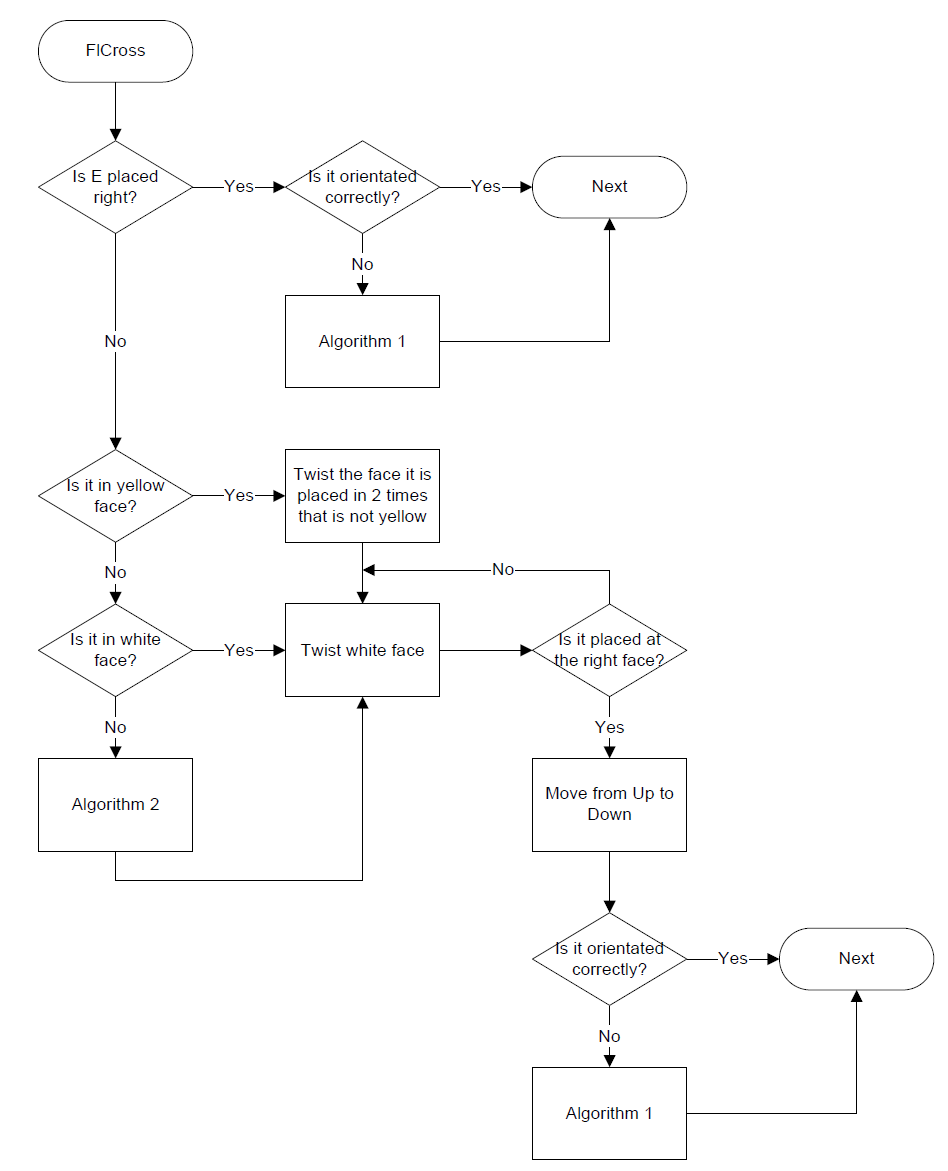
\includegraphics[width = \textwidth]{input/pics/FlCrossFlow3.png}
	\caption{\myCaption{The picture illustrates what is done in step one.}}
	\label{fig:FlCrossFlow}
\end{figure}

